\documentclass[11pt,a4paper]{article}

\usepackage[T1]{fontenc}
\usepackage[utf8]{inputenc}
\usepackage{lmodern}
\usepackage[a4paper,top=2.2cm,bottom=2.2cm,left=2.2cm,right=2.2cm]{geometry}
\usepackage{microtype}
\usepackage{amsmath,amssymb}
\usepackage{booktabs}
\usepackage{graphicx}
\usepackage{xcolor}
\usepackage{caption}
\usepackage{enumitem}
\usepackage[hidelinks]{hyperref}
\usepackage{float}
\usepackage{needspace}

\captionsetup{font=small,labelfont=bf}
\setlist{itemsep=2pt,topsep=3pt}
\renewcommand{\arraystretch}{1.12}
\setlength{\parskip}{2pt}

\newcommand{\fs}{f_s}
\newcommand{\Rnyq}{R_{\mathrm{nyq}}}
\newcommand{\vmax}{v_{\max}}
\newcommand{\dR}{\Delta R}
\newcommand{\CPI}{\mathrm{CPI}}
\newcommand{\dB}{\,\mathrm{dB}}

\title{\vspace{-1.2cm}\textbf{Automotive Waveform for the 1153\,nm FMCW Lidar}\\[4pt]
\large Design note --- proposal for external review}
\author{Range--Doppler chain: HLS central controller + Versal AI Engine}
\date{13 November 2026}

\begin{document}
\maketitle
\vspace{-0.6cm}

\begin{center}
\fbox{\parbox{0.94\linewidth}{\small
\textbf{Goal.} Keep the existing $2048\times256$ range--Doppler chain, but make
the waveform usable at automotive speeds: \textbf{100\,m unambiguous range and
30\,m/s unambiguous velocity at that range}, with $\approx5$\,cm range
resolution.\\[2pt]
\textbf{Status.} Analysis and simulation only. Nothing here has been run on
hardware; the only measured numbers are those of the \emph{current} waveform
(1\,GHz / 2\,GS/s), which are marked as such.}}
\end{center}

\section{Summary}

The present chain measures $\pm0.281$\,m/s unambiguously. That is not a tuning
problem, it is structural:
\begin{equation}
\vmax^{\text{(slow)}} = \frac{\lambda}{4T} = \frac{\lambda \fs}{4 N_{\text{range}}}.
\end{equation}
Bandwidth does not appear in it. Reaching 30\,m/s with chirp-to-chirp Doppler
would need $\fs = 213$\,GS/s, i.e.\ $T = 9.6$\,ns, which is not a lidar front
end. Increasing bandwidth and chirp time---the obvious first move---improves
range resolution but \emph{reduces} the velocity span.

The proposal is to alternate the slope sign every chirp and measure the Doppler
shift of the beat itself. The velocity span then comes from $\fs$ and not from
$T$:
\begin{equation}
\vmax(R) = \frac{\lambda \fs}{2}\,\min(r,\,1-r), \qquad r = \frac{R}{\Rnyq},
\end{equation}
a \emph{triangular} envelope peaking at $\lambda\fs/4$ at half the unambiguous
range.

Recommended point for 100\,m / 30\,m/s / $\approx5$\,cm:
\begin{center}
\fbox{\parbox{0.86\linewidth}{\centering
$B = 2.907$\,GHz, \quad $\fs = 0.98$\,GS/s, \quad $T = 2.090\,\mu$s,\quad
$\dR = 5.16$\,cm,\quad $\Rnyq = 105.6$\,m,\\
$\vmax(100\,\mathrm{m}) = 30.0$\,m/s,\quad peak $282.5$\,m/s at $52.8$\,m.}}
\end{center}
The slow-time FFT is kept: its phase progression across chirps is independent
of the slope sign, so it still supplies $\approx1.1$\,mm/s fine resolution. The
dual-slope estimate only has to be good enough to unwrap it.

The cost is two sub-frames per CPI, up/down peak pairing (ghost risk in dense
scenes), a 2.9\,GHz sweep at 1153\,nm, and almost no margin at exactly 100\,m.

\section{Where the design starts}

The implemented chain is an 11-port HLS kernel feeding an AIE 2048-point range
FFT ($\mathrm{TP\_SHIFT}=11$), a range threshold, a sparse range cube in DRAM,
a 256-chirp persistence AND, an AIE 256-point Doppler FFT
($\mathrm{TP\_SHIFT}=4$), a Doppler threshold and a sparse Doppler cube. FFT
sizes and the dataflow are fixed constraints.

\begin{table}[h]
\centering
\small
\begin{tabular}{@{}lr@{}}
\toprule
Parameter & Value \\
\midrule
Wavelength & 1153\,nm \\
Sweep bandwidth $B$ & 1.0\,GHz \\
Sample rate $\fs$ & 2\,GS/s \\
Samples per chirp & 2048 \\
Chirp time $T$ & 1.024\,$\mu$s \\
Chirps per CPI & 256 \\
CPI & 262.1\,$\mu$s \\
Range resolution $c/2B$ & 14.99\,cm \\
Max unambiguous range & 307.0\,m \\
Velocity resolution $\lambda/(2\,\CPI)$ & 2.199\,mm/s \\
\textbf{Unambiguous velocity $\lambda/(4T)$} & \textbf{$\pm0.281$\,m/s} \\
\bottomrule
\end{tabular}
\caption{Current waveform. The moving-scene test (44.97\,m, 14.07\,cm/s) passes
at $0.999999998$ correlation against the golden fixed-point model; that
verifies the chain, not the waveform.}
\end{table}

\section{Why bandwidth cannot fix the velocity span}

Per chirp the beat frequency of a target at range $R$ is
\begin{equation}
f_R = \frac{2BR}{cT},
\end{equation}
and motion adds a Doppler shift $f_D = 2v/\lambda$ on top of it. Chirp to chirp
the phase of the range-compressed signal advances by
\begin{equation}
\Delta\varphi = \frac{4\pi vT}{\lambda}
\quad\Longrightarrow\quad
\vmax^{\text{(slow)}} = \frac{\lambda}{4T} = \frac{\lambda \fs}{4N_{\text{range}}}.
\end{equation}

\begin{table}[h]
\centering
\small
\begin{tabular}{@{}rrrr@{}}
\toprule
$\fs$ & $T$ & $\vmax$ (slow) & velocity resolution \\
\midrule
1\,GS/s & 2.048\,$\mu$s & 0.141\,m/s & 1.10\,mm/s \\
2\,GS/s & 1.024\,$\mu$s & 0.281\,m/s & 2.20\,mm/s \\
5\,GS/s & 0.410\,$\mu$s & 0.704\,m/s & 5.50\,mm/s \\
10\,GS/s & 0.205\,$\mu$s & 1.407\,m/s & 11.0\,mm/s \\
\bottomrule
\end{tabular}
\caption{Slow-time span versus ADC rate, from \texttt{tb/waveform\_optimizer.py}.
A 10\,GS/s ADC still gives only 1.4\,m/s and degrades the resolution; 30\,m/s
would need 213.1\,GS/s.}
\end{table}

Bandwidth buys range resolution and nothing else here; chirp time actively
works against velocity. The span has to come from the beat frequency itself.

\section{Dual slope}

\subsection{The two measurements}
Send an up-chirp, then a down-chirp of equal duration and bandwidth. For an
approaching target,
\begin{equation}
f_{\text{up}} = f_R - f_D, \qquad f_{\text{down}} = f_R + f_D,
\end{equation}
hence
\begin{equation}
R = \frac{cT\,(f_{\text{up}}+f_{\text{down}})}{4B},
\qquad
v = \frac{\lambda\,(f_{\text{down}}-f_{\text{up}})}{4}.
\end{equation}
Both tones are measured in the same 2048-point range FFT. Their separation is
$2f_D = 104$\,MHz at 30\,m/s, i.e.\ about 217 bins or 11.2\,m---large, and the
main implementation problem (\S\ref{sec:chain}).

\begin{figure}[h]
\centering
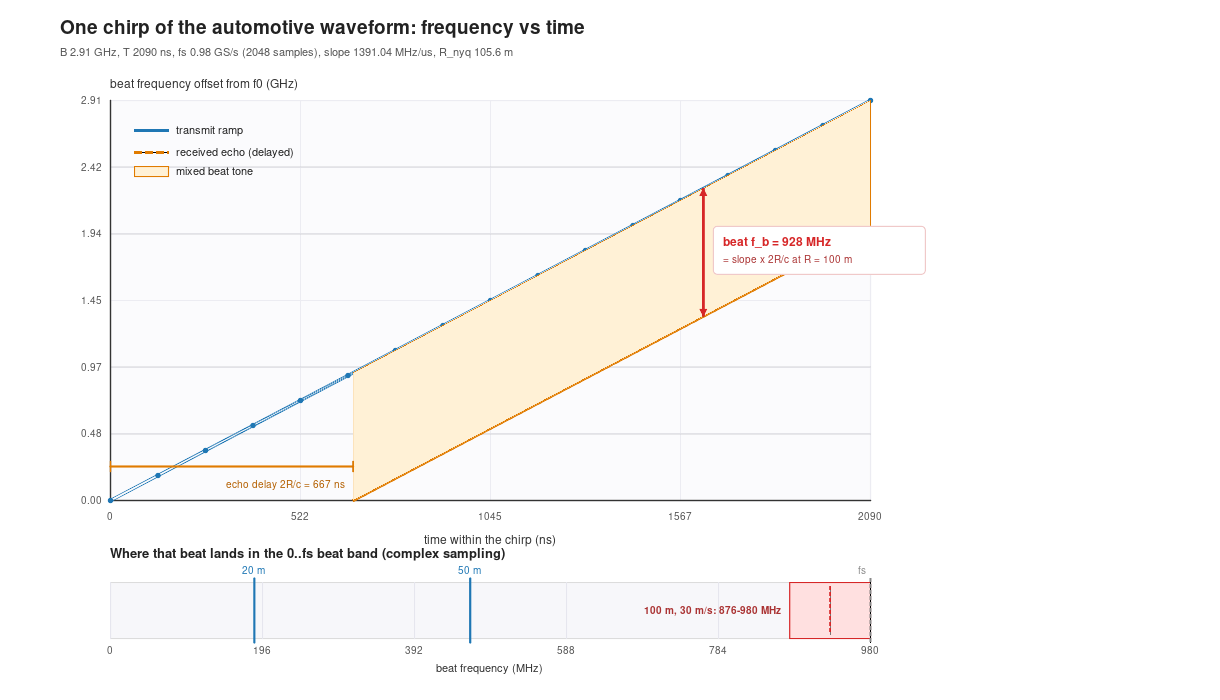
\includegraphics[width=0.92\linewidth]{img/waveform_chirp.png}
\caption{One up-chirp: 2.91\,GHz in 2.09\,$\mu$s. The echo from 100\,m arrives
$2R/c=667$\,ns late, so the mixer output is a tone at 928\,MHz. The next chirp
mirrors the ramp.}
\end{figure}

\begin{figure}[h]
\centering
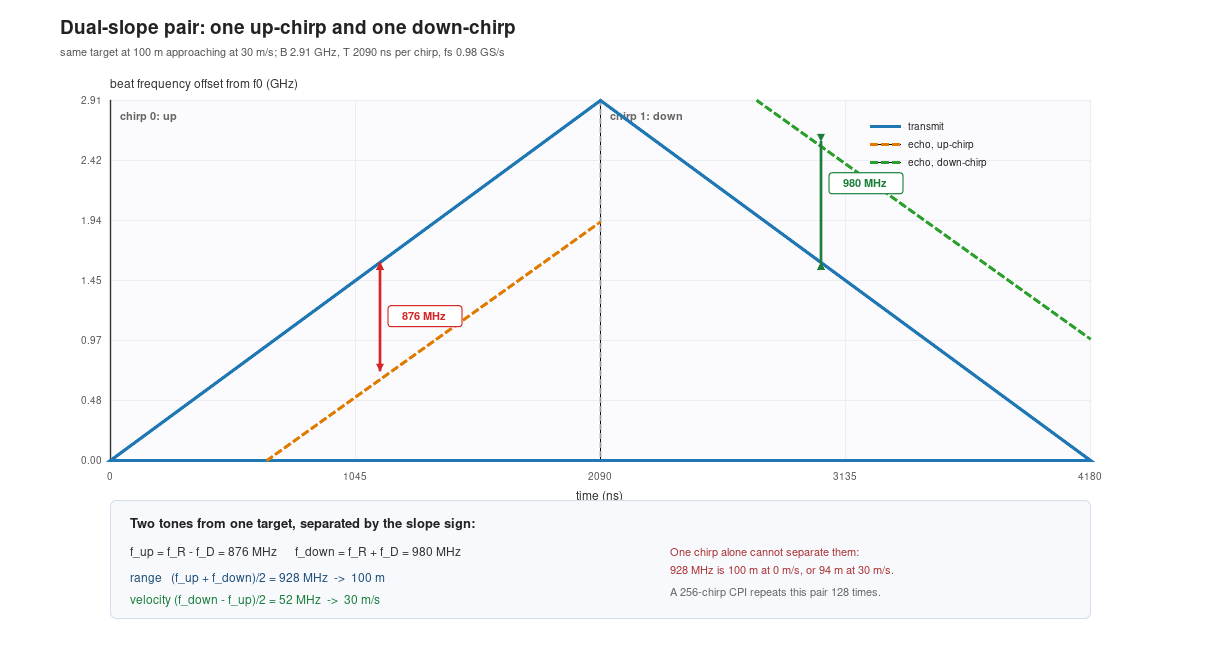
\includegraphics[width=0.92\linewidth]{img/waveform_pair.png}
\caption{The pair: chirp 0 up, chirp 1 down, repeated 128 times per CPI. At
100\,m and 30\,m/s the beats are 876\,MHz and 980\,MHz; their average gives
range, their difference gives velocity.}
\end{figure}

\subsection{The envelope, and why it is triangular}
With complex (I/Q) sampling the beat must stay in $[0,\fs]$:
\begin{equation}
0 \le f_R - f_D \;\Rightarrow\; f_D \le f_R,
\qquad
f_R + f_D \le \fs \;\Rightarrow\; f_D \le \fs - f_R .
\end{equation}
Therefore
\begin{equation}
f_D \le \min(f_R,\fs-f_R)
\quad\Longrightarrow\quad
\boxed{\;\vmax(R) = \frac{\lambda\fs}{2}\min(r,1-r),\quad r=\frac{R}{\Rnyq}\;}
\end{equation}
The envelope peaks at $\lambda\fs/4$ at $R=\Rnyq/2$ and collapses to zero at
both ends of the window. This is the fundamental price of the method:
\textbf{high velocity is only unambiguous in the middle of the range window.}
At the recommended point the peak is 282.5\,m/s at 52.8\,m, 30.0\,m/s at
100\,m, 53.5\,m/s at 10\,m and 5.3\,m/s at 1\,m.

\subsection{The ambiguity it removes}
A single slope gives one number, 928\,MHz at 100\,m, which is 100\,m at 0\,m/s
or 94.4\,m at 30\,m/s. The coupling is
\begin{equation}
\delta R = \frac{v\,cT}{\lambda B} = 5.61\ \mathrm{m}\ \text{at } 30\ \mathrm{m/s},
\end{equation}
so the up/down average cancels it and the difference measures it. Range--Doppler
coupling is not a nuisance to correct afterwards; it \emph{is} the velocity
measurement.

\section{Hybrid: coarse dual, fine slow time}

The dual estimate is coarse, the slow-time phase is fine but aliased; use the
first to unwrap the second.

\begin{itemize}
\item The slow-time phase across chirps is $4\pi vT/\lambda$ \emph{regardless of
the slope sign}, because it is the carrier phase, not the modulation. The
existing 256-point Doppler FFT therefore still produces a fine axis with
$\Delta v = \lambda/(2\,\CPI)$.
\item Its span is $\pm\lambda/(4T) = \pm0.138$\,m/s, i.e.\ 1.078\,mm/s per cell
for 256 chirps.
\item The dual estimate over 128 pairs has a coarse resolution of order
$\lambda/(2T)/\sqrt{128} = 24.4$\,mm/s (a scaling estimate, not a CRLB), which
is $5.7\times$ smaller than the $\pm69$\,mm/s half-span it must unwrap.
\end{itemize}

The same quantity appears twice---$f_D$ as a beat shift and $f_D$ as a
slow-time phase slope. That redundancy is the whole point.

\section{Sizing the waveform}

\subsection{Constraint solve}
For a required velocity $v$ at reference range $R_{\text{ref}}$, with
$x=R_{\text{ref}}/\Rnyq$:
\begin{equation}
x \ge q \ \text{ and }\ 1-x \ge q, \qquad q = \frac{2v}{\lambda\fs},
\qquad\Longrightarrow\qquad q \le x \le 1-q .
\end{equation}
The largest useful bandwidth puts the reference range at the top edge,
$x=1-q$:
\begin{equation}
B_{\max} = \frac{N_{\text{range}}\,c\,(1-q)}{2R_{\text{ref}}},
\end{equation}
capped by $\Rnyq \ge R_{\min}$ and by the laser bandwidth. This is exactly
\texttt{b\_for\_dual()} in the optimizer.

\subsection{Pareto front}

\begin{table}[H]
\centering
\small
\begin{tabular}{@{}rrrrrrrr@{}}
\toprule
$\fs$ (GS/s) & $B$ (GHz) & $T$ (ns) & $\Rnyq$ (m) & $\dR$ (cm) &
$v_{100}$ (m/s) & peak $v$ & $\Delta v$ hybrid \\
\midrule
0.25 & 2.43 & 8192 & 126.3 & 6.17 & 30.0 & 72.1 & 0.27\,mm/s \\
0.49 & 2.75 & 4138 & 111.7 & 5.46 & 30.0 & 142.7 & 0.54\,mm/s \\
\textbf{0.98} & \textbf{2.91} & \textbf{2090} & \textbf{105.6} & \textbf{5.16}
  & \textbf{30.0} & \textbf{282.5} & \textbf{1.08\,mm/s} \\
1.94 & 2.99 & 1056 & 102.8 & 5.02 & 30.0 & 559.3 & 2.13\,mm/s \\
3.84 & 3.03 & 533 & 101.4 & 4.95 & 30.0 & 1107 & 4.22\,mm/s \\
7.99 & 3.05 & 256 & 100.7 & 4.91 & 30.0 & 2302 & 8.78\,mm/s \\
\bottomrule
\end{tabular}
\caption{Bandwidth is essentially pinned near 3\,GHz by the 100\,m / 30\,m/s
constraint; the ADC rate then trades velocity headroom against CPI and
resolution.}
\end{table}

\begin{figure}[H]
\centering
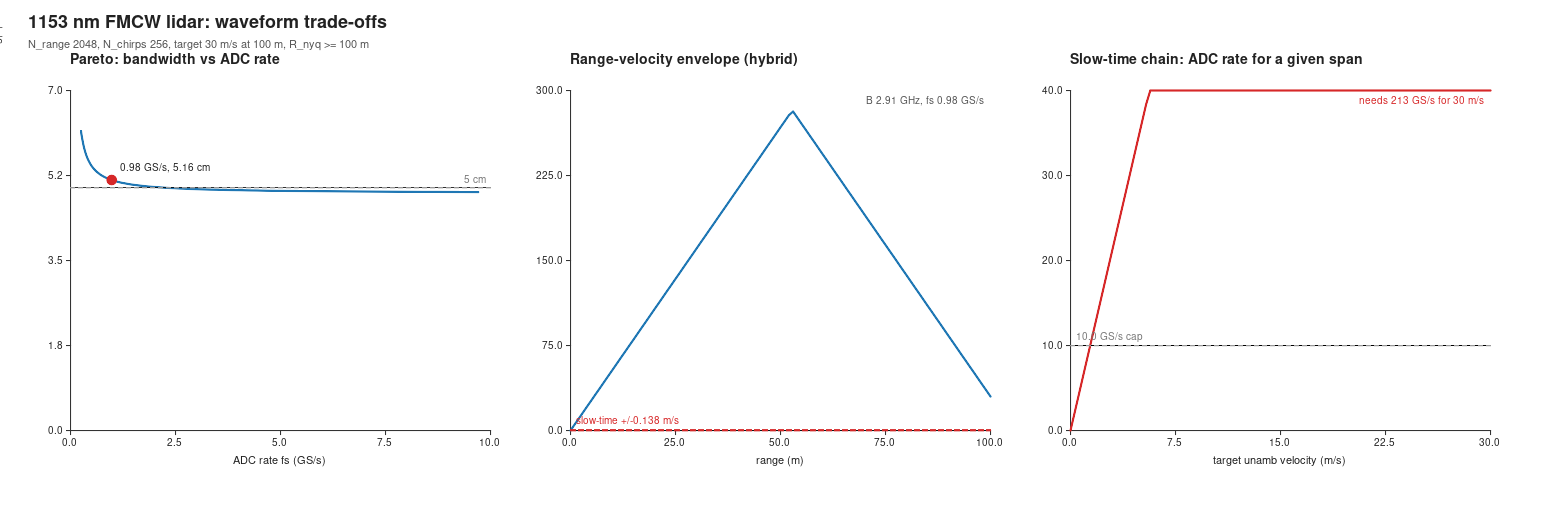
\includegraphics[width=0.95\linewidth]{img/waveform_tradeoffs.png}
\caption{Design space: range resolution versus ADC rate, the triangular
velocity envelope, and the ADC rate the slow-time chain would need.}
\end{figure}

The minimum-rate design still meeting 6\,cm is 0.29\,GS/s, 2.52\,GHz,
7.08\,$\mu$s, but its peak envelope is only 83.6\,m/s.

\Needspace{18\baselineskip}
\subsection{Recommended point}

\begin{table}[H]
\centering
\small
\begin{tabular}{@{}lr@{}}
\toprule
Quantity & Value \\
\midrule
Bandwidth & 2.907\,GHz \\
Range resolution & 5.156\,cm \\
Nyquist range & 105.61\,m \\
Sample rate & 0.980\,GS/s \\
Chirp time & 2.0898\,$\mu$s \\
Slope & 1.391\,MHz/$\mu$s \\
CPI (256 chirps) & 535.0\,$\mu$s \\
Range bin & 478.5\,kHz / 5.156\,cm \\
$\vmax$ at 100\,m & 30.0\,m/s \\
Peak $\vmax$ (52.8\,m) & 282.5\,m/s \\
$\vmax$ at 10\,m & 53.5\,m/s \\
Doppler shift at 30\,m/s & 52.0\,MHz = 108.7 bins \\
Range--Doppler coupling at 30\,m/s & 5.61\,m \\
Fine $\Delta v$ (slow time, 256 chirps) & 1.078\,mm/s \\
Coarse dual $\Delta v$ (128 pairs) & $\approx$24.4\,mm/s \\
Physical migration in one CPI at 30\,m/s & 1.6\,cm (0.31 bin) \\
\bottomrule
\end{tabular}
\caption{Recommended point. The last line matters: range walk within the CPI is
negligible; what moves the peak between up and down chirps is the Doppler shift
of the beat, not target motion.}
\end{table}

\Needspace{14\baselineskip}
\subsection{Sensitivity}
Each 1\,m/s of extra velocity at 100\,m costs about 5.4\,MHz of bandwidth:

\begin{table}[H]
\centering
\small
\begin{tabular}{@{}rrrrr@{}}
\toprule
$v$ at 100\,m & $B$ & $\Rnyq$ & $\dR$ & peak $v$ \\
\midrule
30\,m/s & 2.907\,GHz & 105.6\,m & 5.16\,cm & 282.5\,m/s \\
35\,m/s & 2.880\,GHz & 106.6\,m & 5.21\,cm & 285.6\,m/s \\
40\,m/s & 2.852\,GHz & 107.6\,m & 5.25\,cm & 288.6\,m/s \\
\bottomrule
\end{tabular}
\caption{Since 30\,m/s at 100\,m lands exactly on the envelope, sizing for
35\,m/s costs only 0.5\,\% of range resolution.}
\end{table}

\section{What this does to the implemented chain}
\label{sec:chain}

\subsection{Range path}
Unchanged: 2048 samples, Hamming, AIE 2048-point FFT, 16-bin block threshold,
persistence AND, sparse cube. Only the bin meaning changes: 5.156\,cm per bin
instead of 14.99\,cm; a 16-bin threshold block is 82.5\,cm instead of 2.4\,m;
$\Rnyq$ drops from 307\,m to 105.6\,m, so the mask covers 105.6\,m with the
same 128 blocks (0.825\,m per block). The block-mean statistics still apply,
but the Gamma(16) assumption and the median/mode fit now see a much finer
range sampling; the false-alarm rate should be re-measured on the
\texttt{dense} scene.

\subsection{Doppler path --- the real problem}
If the slope alternates every chirp, then for a moving target the range peak
alternates between $f_R-f_D$ and $f_R+f_D$, i.e.\ between bins 217 apart. The
256-chirp Doppler FFT would see a signal jumping between two range bins, which
breaks the slow-time sequence for that bin. Three options:

\begin{enumerate}[label=\arabic*.]
\item \textbf{Two sub-frames (recommended).} Treat up-chirps and down-chirps as
two 128-chirp sequences, each with its own range mask, persistence AND and
Doppler pass. The 256-point AIE FFT can process 128 real chirps zero-padded, so
the IP does not change; the Doppler pass runs twice per block, doubling that
part of the compute and the Doppler read/write traffic.
\item \textbf{Compensate the range shift before the Doppler FFT.} Requires
knowing $f_D$ to shift each chirp's spectrum back---a two-pass scheme (coarse
estimate, then realign) with a feedback path through DRAM.
\item \textbf{Skip the per-chirp range FFT for the Doppler stage.} Estimate
$f_D$ first, then do one corrected Doppler FFT. Cleaner mathematically, but it
discards the sparse-cube architecture.
\end{enumerate}

Option 1 preserves the block/AND/threshold structure and makes the two
measurements independent. The AND then spans 128 chirps instead of 256, so it
is slightly less selective; the moving scene's 21.4\,\% Doppler write fraction
should be re-measured and will probably rise.

\subsection{Pairing and ghosts}
With several targets the up and down frames each produce peaks. A pair is the
same target if
\begin{equation}
|R_{\text{up}}-R_{\text{down}}| = 2\delta R\,(v/30) \quad\text{and}\quad
|v_{\text{up}}| = |v_{\text{down}}| .
\end{equation}
Nearest-neighbour pairing works for one target and for well separated ones; in
a dense scene it produces ghosts, exactly like a range--Doppler MIMO pairing
problem. Mitigations, in increasing cost: constrain the search by the predicted
11.2\,m offset; require both peaks to share a Doppler cell; add a third slope
to over-determine the fit; or rely on the upstream point-cloud tracker. This is
the biggest algorithmic hole in the proposal and needs a dedicated simulation
with two to four targets.

\subsection{Thresholds, DRAM and fixed point}
Same cube layout, same 128 sequences, same sparse cubes. The Doppler median is
unaffected by the slope sign, but each pass now has 128 samples instead of 256,
so the median is noisier and the $10^{8.393/10}$ constant should be re-checked.
$\mathrm{TP\_SHIFT}$ does not depend on the slope; $f_D=52$\,MHz is 108 bins at
478.5\,kHz, so there is no resolution pressure on the range FFT. Window, mask
width and 16-bin write granularity are unchanged.

\section{Validation plan}

Cheap, in order, before any hardware:
\begin{enumerate}[label=\arabic*.]
\item Extend the physical scene generator to the new parameters and a 100\,m,
30\,m/s target; check the range peak lands near bin 1939 and the Doppler peak
matches the aliasing formula.
\item Build a Python dual-slope model: split chirps, two range FFTs, threshold,
pairing, $R$/$v$ estimate; compare with truth for 1, 2 and 4 targets.
\item Run the same scene through the fixed-point golden model to confirm the
slow-time phase really is slope-independent after the hardware shifts.
\item Measure the pairing ghost rate versus target density and SNR; this
decides whether option 1 suffices.
\item Re-measure threshold selectivity and DRAM traffic for 128-chirp
sub-frames.
\item Only then size the laser: 2.9\,GHz of linear sweep in 2.09\,$\mu$s at
1153\,nm, with coherence over the CPI.
\end{enumerate}

\section{Questions for the reviewer}

\begin{enumerate}[label=\textbf{Q\arabic*.}]
\item Is the triangular envelope derivation right for this front end? It
assumes complex sampling over $[0,\fs]$ and a real, positive beat. With real
sampling the envelope halves.
\item Is per-slope sub-framing (\S\ref{sec:chain}) the right call, or is a
two-pass range-shift compensation worth the DRAM round trip?
\item How would you pair up/down peaks in a dense scene without a tracker? Is a
third slope cheaper than a tracker?
\item 30\,m/s at 100\,m sits exactly on the envelope. Size for 35--40\,m/s
(costs $\approx1$\,\% range resolution), or accept a velocity-dependent maximum
range?
\item The near-range envelope collapses (5.3\,m/s at 1\,m). Acceptable for an
automotive sensor, or does it force a second, shorter waveform?
\item The coarse dual resolution ($\approx$24\,mm/s) is a scaling estimate.
What is the realistic CRLB at 10\,dB SNR, and does the unwrap still hold?
\item Is a 2.9\,GHz sweep realistic for a 1153\,nm source (coherence,
linearity, modulator bandwidth), or does this silently require another laser?
\item Does anything in the fixed-point chain break when the chirps per Doppler
pass halve?
\end{enumerate}

\appendix
\section{Formulas}

\begin{align}
f_R &= \frac{2BR}{cT}, &
f_D &= \frac{2v}{\lambda}, &
\Rnyq &= \frac{N_{\text{range}}c}{2B}, \\
\dR &= \frac{c}{2B}, &
T &= \frac{N_{\text{range}}}{\fs}, &
\vmax^{\text{(slow)}} &= \frac{\lambda\fs}{4N_{\text{range}}}, \\
\Delta v_{\text{slow}} &= \frac{\lambda}{2N_{\text{chirps}}T}, &
\vmax(R) &= \frac{\lambda\fs}{2}\min\!\left(\frac{R}{\Rnyq},1-\frac{R}{\Rnyq}\right), &
\delta R &= \frac{v\,cT}{\lambda B}.
\end{align}

\section{Numbers at the recommended point}
\begin{center}
\small
\begin{tabular}{@{}llll@{}}
\toprule
$\lambda = 1153$\,nm & $B = 2.9068$\,GHz & $\fs = 0.980$\,GS/s &
$T = 2.0898\,\mu$s \\
$N_{\text{range}} = 2048$ & $N_{\text{chirps}} = 256$ &
$\dR = 5.156$\,cm & $\Rnyq = 105.61$\,m \\
$f_{\text{bin}} = 478.5$\,kHz & $\CPI = 535.0\,\mu$s &
$\vmax(100) = 30.0$\,m/s & $v_{\text{peak}} = 282.5$\,m/s \\
$\Delta v_{\text{slow}} = 1.078$\,mm/s & $f_D(30) = 52.04$\,MHz &
$f_{\text{up}} = 876.0$\,MHz & $f_{\text{down}} = 980.0$\,MHz \\
\bottomrule
\end{tabular}
\end{center}

\section{Files}
\begin{center}
\small
\begin{tabular}{@{}p{0.47\linewidth}p{0.47\linewidth}@{}}
\toprule
File & What it does \\
\midrule
\texttt{tb/waveform\_optimizer.py} & design-space sweep, Pareto table, trade-off plot \\
\texttt{tb/waveform\_chirp\_plot.py} & one-chirp frequency--time figure \\
\texttt{tb/waveform\_pair\_plot.py} & up/down pair figure \\
\texttt{tb/rd\_test.py} & scene generator, golden fixed-point model, checks \\
\texttt{src/doppler\_part.cpp} & persistence AND, Doppler threshold \\
\texttt{fft\_accelerator\_component/src/graph.h} & AIE range/Doppler graphs, shifts \\
\bottomrule
\end{tabular}
\end{center}

\vspace{4pt}
\noindent\small The optimizer runs with no arguments for the defaults used
here:
\begin{verbatim}
python3 central-controller-element/tb/waveform_optimizer.py
\end{verbatim}

\end{document}
